% !TeX root = ../main.tex

\chapter{基于深度强化学习的性能驱动集群调度算法}\label{chap:adasched}

针对当前深度学习集群调度器在截止机制和资源分配策略上存在的局限性，
本章提出一种基于深度强化学习的性能驱动调度算法AdaSched。
本章首先分析了现有基于迭代次数的调度截止机制所面临的核心问题，在此基础上给出了性能驱动调度的形式化定义
和优化目标。
随后，详细介绍了AdaSched的整体系统架构与工作流程，并逐一介绍各关键模块的设计原理与实现细节，
包括性能预测模型、基于强化学习的调度器以及策略网络的结构设计。
最后，通过在多组包含真实与合成轨迹的深度学习负载数据集上开展实验，
对比了AdaSched相比于现有前沿算法在各项核心指标上的性能表现。

\section{问题描述}\label{sec:problem}

\subsection{问题背景}\label{subsec:problem-bg}

本文聚焦于多租户共享的同构 GPU 集群环境。在该系统中，深度学习训练作业随时间持续到达，
且所有作业均采用数据并行的方式进行分布式训练。
在该环境下，集群采用弹性训练机制，允许作业在不同的资源配置下灵活地挂起和恢复，从而充分利用集群资源。

如第\ref{chap:related-work}章所述，现有的集群调度器通常依赖用户指定的最大迭代次数作为作业完成的判定依据。然而，由于用户对模型
收敛行为缺乏精确认知，其对所需迭代次数的估计往往存在较大偏差。这种不准确的估计将导致双重后果：一方面，
低估作业所需的迭代次数可能导致作业在模型尚未充分收敛时过早终止；另一方面，高估作业所需的迭代次数则会
导致作业在性能目标已达成后仍持续占用计算资源，造成严重的资源浪费。

在具有截止期限约束的深度学习训练作业调度场景下，上述问题尤为突出。
当前先进的截止期限感知调度器（如Chronus和ElasticFlow）均采用准入控制机制来保障作业按时完成，
其通过预测作业能否在截止期限前完成全部指定迭代次数来决定是否接纳该作业。因此，
高估作业的迭代次数将增大该作业被准入控制模块拒绝的概率，导致大量原本可以在截止期限内达到期望性能水平的作业被不合理地拒
绝，最终降低了用户满意度和集群吞吐量。

实际上，用户的主要关注点在于训练得到的模型性能是否满足其需求，而指定的迭代次数仅是其对达到
训练目标所需资源量的粗略估计。
针对系统优化目标与用户实际需求不匹配的问题，本文提出以性能目标代替迭代次数作为作业完成的主要判定依据，
从而将确定性能目标与所需迭代次数之间的映射关系这一复杂任务从用户端转移至调度端。

\subsection{多级性能目标机制}\label{subsec:multi-level}

在实际生产环境中，模型的实用价值并非由单一的性能指标所决定：较低精度的模型虽不足以直接部署上线，但完全可支撑快速的原型验证或消融实验；
而高性能模型则专用于核心线上服务。
然而，现有调度器大多将单一收敛指标作为作业完成的唯一判据。这种“全有或全无”的
二元调度逻辑，结合集群所采用的准入机制，极易导致部分无法完全收敛但仍具工程价值的作业被拒绝。为了适配
模型用途的多样性，本文主张调度器需打破单一目标的限制，允许用户根据具体需求声明灵活的多级性能目标。
例如，用户可在提交作业时同时设定99\%的理想准确率和98.5\%的可接受目标。
在此范式下，各级性能目标对应不同的资源预算，调度器需要能够根据实时集群资源利用情况，
自适应地为作业选择当前条件下可达的最优性能目标，同时确保作业在截止期限内完成。

相较于传统的二元可行性判定，该机制将调度决策过程从简单的“全有或全无”判断转变为从一组备选方案中
寻求最优结果的过程，从而提升集群的作业准入率、GPU 资源利用率以及调度吞吐量。

为从数学层面支撑这一动态决策机制，本文为调度器设计了一个调度回报函数。该函数将作业的每种性能水平映射为特定的调度回报，
从而将复杂的、多目标的调度过程转化为一个旨在最大化集群全局累计调度回报的经典优化问题。

采用这种自适应调度范式引入了两个核心挑战：
\begin{itemize}
  \item 决策空间极度庞大。调度器需要根据集群状态，选择每个作业合适的性能目标，
        并以此确定每个作业的资源分配方案，这使得调度的复杂度远高于传统的调度场景。
  \item 模型性能与训练迭代次数之间通常遵循非线性关系，具有明显的边际收益递减特征。随着训练的推进，等量计算资源带来的性能增益持续缩小。
        这种非线性且随训练进度不断变化的资源-性能转化率，极大地增加了调度算法在精准评估决策收益与制定最优策略时的难度。
\end{itemize}

为了应对以上挑战，本文设计了一种基于深度强化学习的GPU集群调度算法，AdaSched。
本节首先给出该动态调度范式问题的形式化定义，随后介绍AdaSched的具体框架与算法设计。

\subsection{问题定义}\label{subsec:formulation}

\begin{table}
  \centering
  \caption{问题定义相关符号表}
  \begin{tabular}{ll}
    \toprule
    符号                      & 定义                                               \\
    \midrule
    $G$                     & 集群总GPU数量                                         \\
    $N$                     & 待处理作业数量                                          \\
    $L$                     & 系统允许的最大性能目标级数                                          \\
    $D_i$                   & 作业$i$的截止期限                                       \\
    $E_i$                   & 作业$i$的最大迭代次数                                     \\
    $f$                     & 调度回报函数                                             \\
    $s_{i,l}$               & 作业$i$是否达到第$l$级性能水平                               \\
    $R_{i,l}$               & 作业$i$在第$l$级性能水平下的调度回报                            \\
    $E_{i,l}$               & 作业$i$达到第$l$级性能水平所需的迭代次数                           \\
    $g_{i,t}$               & 作业$i$在时间片$t$分配的GPU数量                             \\
    $p_{i,t}$               & 作业$i$在时间片$t$的放置策略                                \\
    $O_i\left(g_{i,t}, p_{i,t}\right)$ & 作业$i$在时间片$t$给定资源分配$g_{i,t}$和放置策略$p_{i,t}$下的训练吞吐量 \\
    $T_i$                   & 作业$i$的可用总调度时间片数                                  \\
    $st_i$                  & 作业$i$的提交时间                                       \\
    $I$                     & 调度间隔时长                                           \\
    \bottomrule
  \end{tabular}
  \label{tab:chapter3-1}
\end{table}

考虑一个总容量为$G$个GPU的同构集群，单个调度轮次中包含$N$个待处理作业。
每个作业$i$关联一个截止期限$D_i$和最大迭代次数$E_i$。由集群管理员定义一个调度回报函数
$f\left(\left\langle M_1, R_1 \right\rangle, \ldots, \left\langle M_l, R_l \right\rangle\right)$来指定作业完成后可获得的回报值，
其中$M_l$表示第$l$级性能指标，$R_l$表示与该指标关联的调度回报，而$E_{i,l} \left(l = 1, \ldots, L\right)$表示作业
$i$达到第$l$级性能目标所需的迭代次数。
图~\ref{fig:return-function} 展示了一个较为合理的调度回报函数设计实例，其中
作业调度回报随模型最终达到的性能水平提升而递增。

\begin{figure}[htbp]
  \centering
  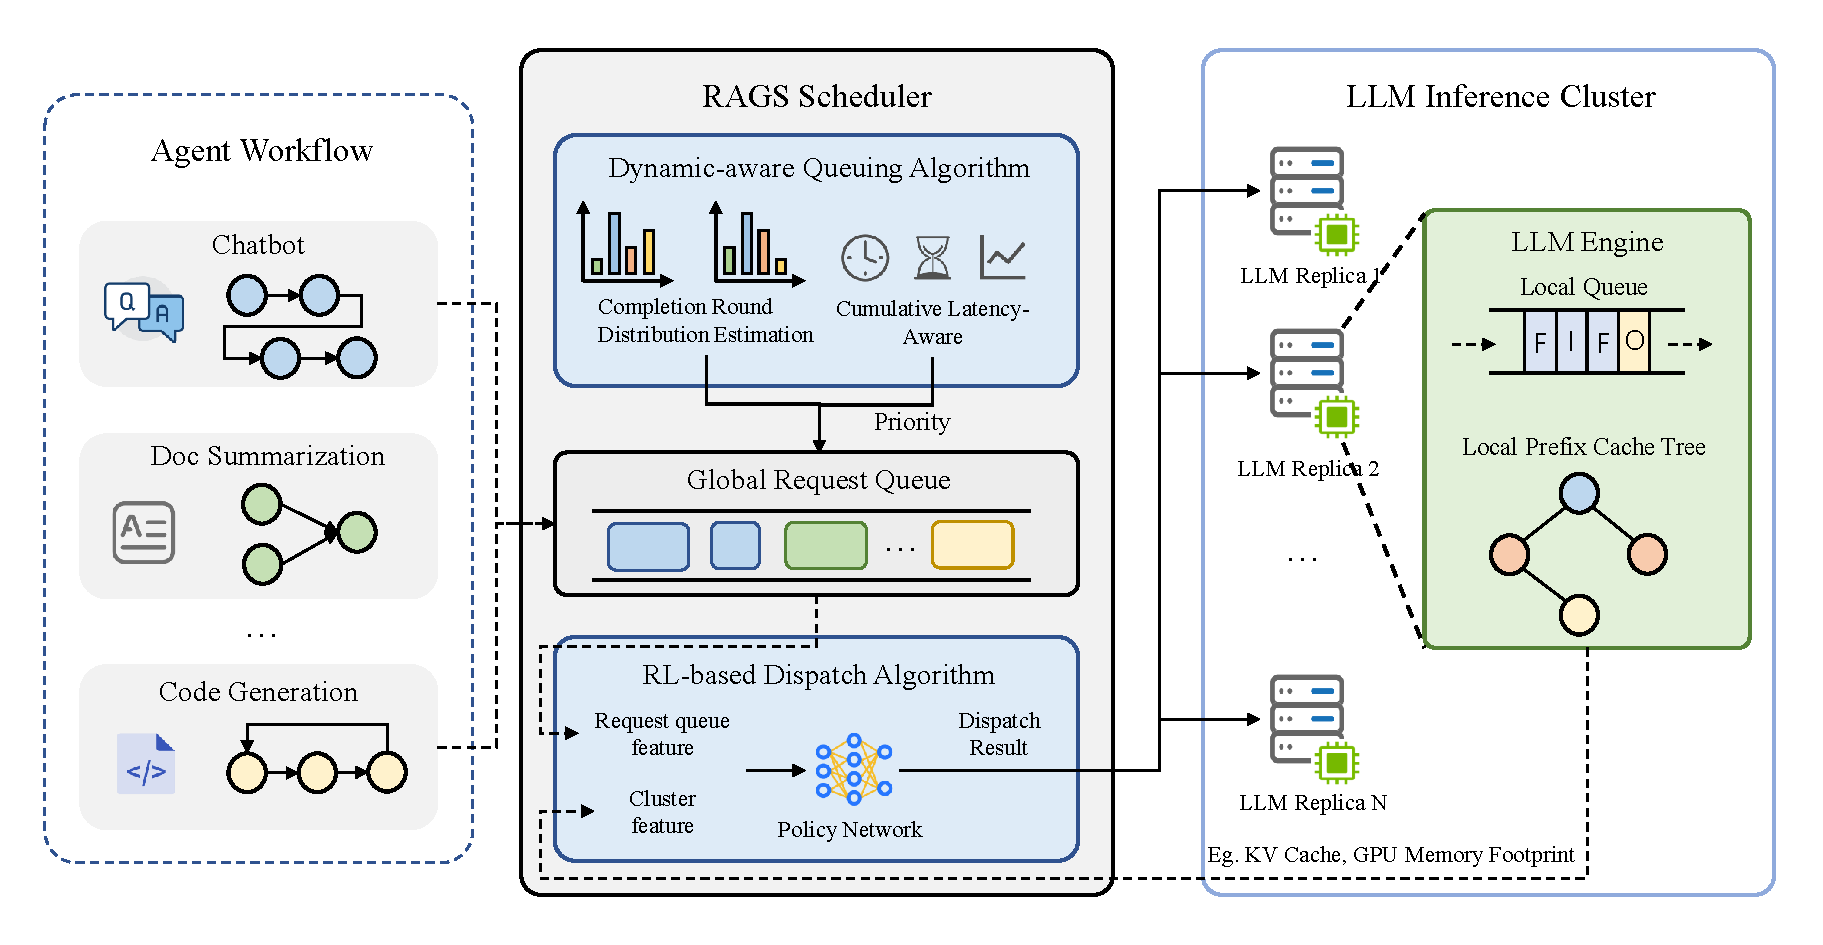
\includegraphics[width=0.6\textwidth]{figures/3.1.pdf}
  \caption{调度回报函数实例示意图}
  \label{fig:return-function}
\end{figure}

集群的优化目标为找到最优的资源分配策略，使所有作业的总调度回报最大化，即：
\begin{equation}\label{eq:objective}
  \max \sum_{i=1}^{N} \sum_{l=1}^{L} s_{i,l} \times R_{i,l},
\end{equation}
其中，二值变量$s_{i,l} \in \left\{0, 1\right\}$表示作业$i$是否达到其第$l$级性能水平。约束(\ref{eq:constraint-one-target})
确保每个作业至多达到一个性能目标：
\begin{equation}\label{eq:constraint-one-target}
  \sum_{l=1}^{L} s_{i,l} \leq 1, \quad s_{i,l} \in \left\{0, 1\right\}, \quad \forall i \in \left\{1, 2, \ldots, N\right\}.
\end{equation}

鉴于系统采用弹性训练范式，在单一调度轮次结束时，所有执行中的作业均会被强制挂起，
并触发检查点机制以持久化其训练状态，其占用的底层 GPU 资源随之被彻底释放。因此，每个调度轮次开始时，集群中所有 GPU 均处于
空闲状态，可供调度器重新统一分配。
约束(\ref{eq:constraint-capacity})保证在每个时间片$t$内，所有作业的资源使用量不超过集群总容量：
\begin{equation}\label{eq:constraint-capacity}
  \sum_{i=1}^{N} g_{i,t} \leq G, \quad \forall t.
\end{equation}

其中$g_{i,t}$表示在时间片$t$为作业$i$分配的GPU数量。进一步地，假设模型性能与训练迭代次数之间的对应关系已知，
则为了获得用户指定的第$l$级性能水平的调度回报，调度器必须确保作业$i$在其截止期限$D_i$前
至少需要完成$E_{i,l}$次迭代：
\begin{equation}\label{eq:constraint-iteration}
  \sum_{t=1}^{T_i} s_{i,l} \times O_i\left(g_{i,t}, p_{i,t}\right) \times I \geq s_{i,l} \times E_{i,l}, \quad \forall i \in \left\{1, 2, \ldots, N\right\}.
\end{equation}

在式(\ref{eq:constraint-iteration})中，$O_i\left(g_{i,t}, p_{i,t}\right)$为作业$i$在时间片$t$给定资源分配$g_{i,t}$和
放置策略$p_{i,t}$下的训练吞吐量，即作业每秒可执行的迭代次数。作业的截止期限$D_i$决定了其可用的总调度时间片
个数$T_i$，计算方式为$T_i = \left\lceil \left(D_i - st_i\right) / I \right\rceil$，其中$st_i$为作业提交时间，
$I$为调度间隔时长。

上述优化目标与约束条件共同构成了一个典型的混合整数线性规划（MILP）问题。尽管在理论上可通过 Gurobi~\cite{gurobi} 
等商用精确求解器获取最优解，但由于弹性调度场景下庞大的决策空间，
该问题极易引发组合爆炸。实验结果（详见第\ref{subsec:experiment-overhead} 节）表明，
传统求解器难以在合理的求解时间内获得高质量的精确解，甚至在极端高负载下无法求得可行解。
另一方面，传统的启发式算法受限于固定的贪婪规则，极易陷入局部最优从而导致次优的调度性能。
因此，本文采用深度强化学习重构调度器的决策核心，旨在利用其强大的状态表征能力与在线推理特性，
在极低的调度延迟下生成逼近全局最优的资源分配策略。

\section{算法设计}\label{sec:architecture}

\subsection{系统架构}\label{subsec:architecture}
AdaSched的整体系统架构如图~\ref{fig:architecture} 所示，其工作流程由以下几个关键阶段组成。

\begin{figure}[htbp]
  \centering
  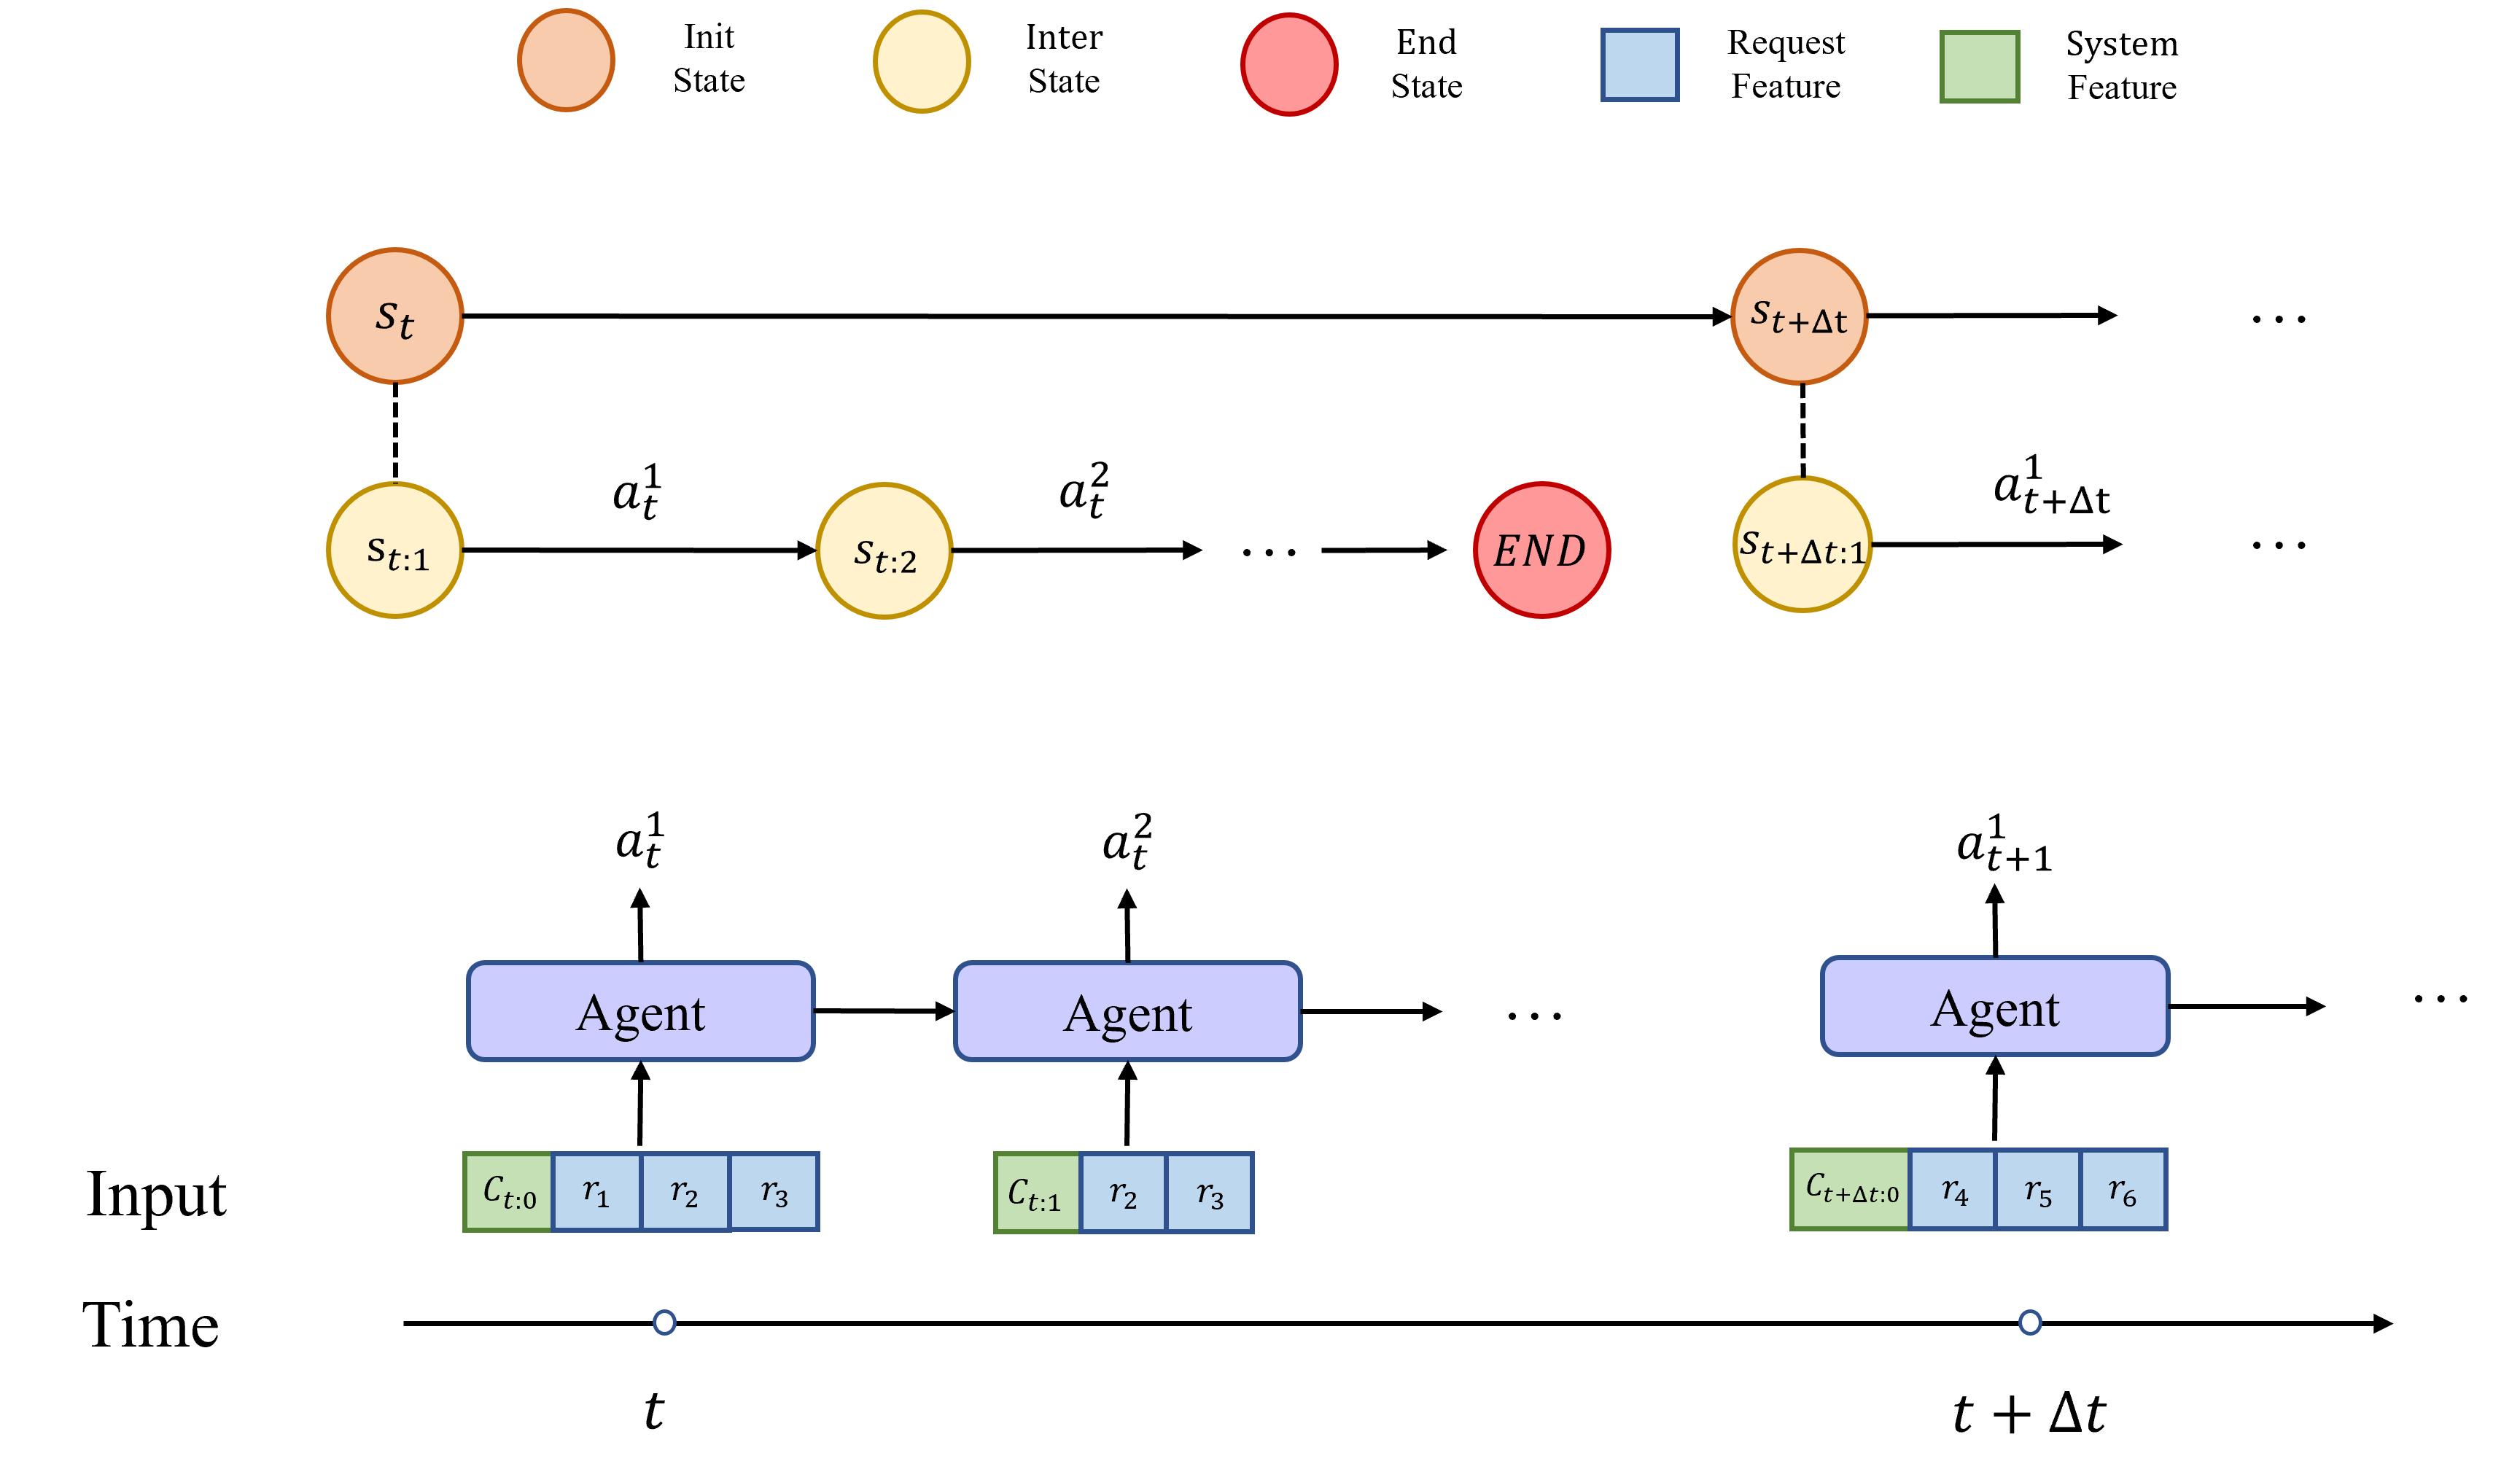
\includegraphics[width=\textwidth]{figures/3.2.png}
  \caption{AdaSched系统架构}
  \label{fig:architecture}
\end{figure}

当用户提交深度学习训练作业时，需声明以下元数据：(1) 模型网络架构（如 VGG、BERT 等）；(2) 期望的截止期限；
(3) 多级性能目标；(4) 最大训练迭代次数。提交后的作业首先被推入待调度队列~\ding{172}。
随后，调度器以固定周期对队列中所有作业的状态特征进行编码，并输入至上下文感知的强化学习智能体中，
以生成全局资源分配策略（\ding{173} 与 \ding{174}）。待分配决策确定后，放置器（Placer）采用通信感知的放置算法，
将作业的计算资源精确映射至底层物理节点~\ding{175}。

在单一调度轮次执行完毕后，系统立即触发检查点机制以持久化各作业当前的训练状态。同步地，性能预测模型动态采集各作业的运行时反馈
（包含已完成迭代步数与当前模型精度等）~\ding{176}。这些动态信息与作业初始元数据相融合，用于拟合各作业未来的完整收敛曲线。
基于该预测曲线与元数据，奖励模块计算出当前轮次的全局奖励信号，进而驱动强化学习策略网络的策略参数更新（\ding{177} 与 \ding{178}）。
最终，达成性能目标或触及迭代上限的作业将被终止并向用户交付结果~\ding{179}；而尚未完成的作业则重新进入待调度队列，
参与下一轮次调度。

\subsection{性能预测模型}\label{sec:performance-model}

性能预测模型是 AdaSched 实现性能驱动调度的基础组件，其主要职责在于预测作业训练相关曲线的未来轨迹。
AdaSched 引入了基于集成学习的开源预测方案~\cite{domhan2015speeding}。具体而言，该预测模块实时提取
作业运行时日志中的关键状态信息（如已完成迭代次数与当前验证指标），动态拟合出作业完整的生命周期性能曲线。
借助这种预测能力，调度器能够提前评估每个作业在不同资源分配方案下可达到的性能水平，
为后续的调度决策提供了定量依据。此外，该预测模块在架构上被设计为可插拔组件，能够无缝替换或集成其他先进的曲线预测算法。

值得注意的是，在吞吐量预测方面，现有工作通常高度依赖外部性能分析器（Profiler）来离线收集数据，
并以此构建繁杂的显式吞吐量模型 $O\left(g, p\right)$。不同于此，AdaSched 通过强化学习智能体与环境的持续交互，
能够隐式捕获并适应底层硬件吞吐特征的变化，从而有效避免了复杂的显式建模开销。
\subsection{基于强化学习的调度器设计}\label{sec:rl-scheduler}

\subsubsection{马尔可夫决策过程建模}\label{subsec:sequential-decision}

将弹性资源分配问题形式化为强化学习过程时，一种直观的建模方式是将所有待处理作业的完整资源分配方案定义
为单步联合动作。然而，该方法会导致动作空间规模高达$\mathcal{O}\left(M^N\right)$（其中$M$为单作业可请求的GPU数量上限，$N$为队列中的作业总数）。
这种随并发作业规模呈指数级爆炸的高维动作空间，极大阻碍强化学习智能体的有效探索与策略的平稳收敛。

为应对这一挑战，AdaSched将全局资源分配重构为序列化决策问题，通过增量式推理的方式逐步构建完整的资源分配方案。
具体而言，系统将单个宏观调度轮次映射为强化学习中的一个完整回合（Episode）。在回合内，调度器通过多步马尔可夫
决策生成最终方案：在每个微观决策步，智能体基于当前集群状态输出一个离散动作，即
为某个特定作业增量分配一个单位的GPU资源。
当全局分配资源耗尽或触发终止条件时，当前回合结束，生成的最终分配策略随后交由底层的放置算法（Placer）执行物理节点映射。

图~\ref{fig:mdp} 展示了该序列化决策的马尔可夫决策过程实例。
在宏观层面，红色节点 $S_i$ 表征第 $i$ 个调度轮次起始时刻的集群初始状态。
在微观层面，单一调度轮次的资源分配过程被解耦为一个完整的序列决策回合。
具体而言，黄色节点 $S_{i:k}$ 代表该回合内的中间状态（其中，初始状态 $S_{i:1}$ 直接由宏观状态 $S_i$ 继承而来）。
在回合内的每个决策步中，强化学习智能体基于当前状态 $S_{i:k}$ 选择动作 $a_{i:k}$（即为索引为 $a_{i:k}$ 
的作业增量分配一个最小单位的计算资源），从而驱动环境向下一状态 $S_{i:k+1}$ 发生转移。
该过程将持续进行直至触发终止条件并到达最终状态（蓝色节点），标志着当前调度轮次全局资源分配策略的正式生成。

\begin{figure}[htbp]
  \centering
  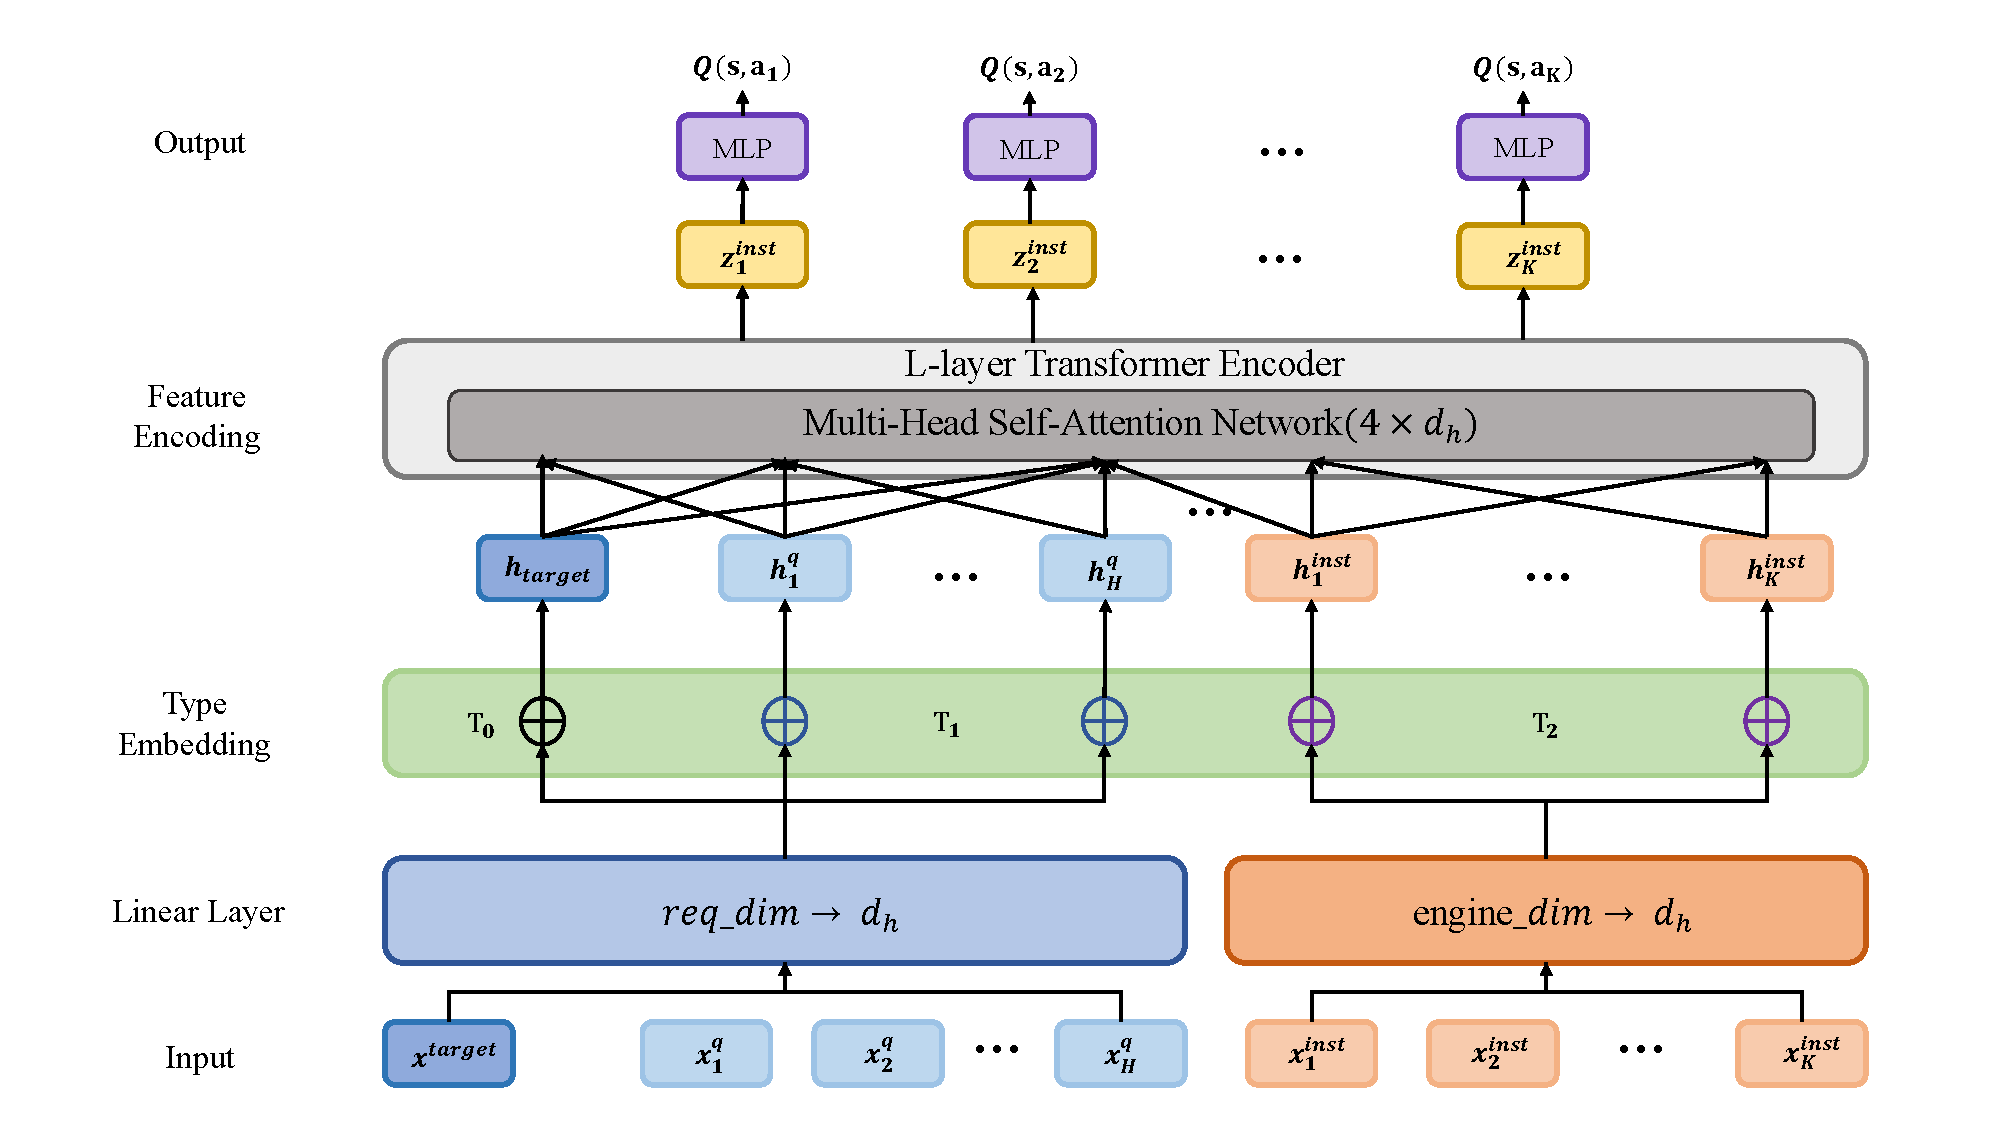
\includegraphics[width=\textwidth]{figures/3.3.png}
  \caption{AdaSched中包含4个作业的马尔可夫决策过程示例}
  \label{fig:mdp}
\end{figure}

上述MDP建模与弹性调度的标准范式相适应。在弹性调度中，集群通过检查点（Checkpoint）技术实现资源的周期性重分配：
在每个调度轮次结束时，未完成的作业会将其最新的训练状态（包括模型参数、优化器状态及训练进度等）持久化至检查点文件（Save），
并主动释放所占用的 GPU 资源以供系统进行全局重分配。
待新一轮分配策略下达后，保留作业将依据最新决策，在相应的物理节点上加载检查点并恢复（Restore）训练。
本文的MDP建模正是对该弹性调度范式的抽象：每个调度轮次对应一个MDP回合，调度器在每轮均可基于最新的集群
状态对底层资源进行重新调配，从而根据作业的最新训练进度和剩余截止时间动态调整分配策略，
避免因沿用上一轮次的陈旧分配方案而导致资源利用率下降。

此外，在某一调度轮次的执行过程中，一旦某作业达成预设性能目标或完成全部训练迭代，系统将立即终止该作业并向用户交付结果，
其释放的 GPU 资源在当前周期剩余时间内会处于短暂的空闲状态。
而其余未完成的作业则在当前周期结束时严格执行上述检查点机制，随后参与下一轮调度。

\subsubsection{状态空间设计}\label{subsec:state}

策略网络的输入状态空间由静态特征与动态特征两部分构成。其中，静态特征在单一调度周期的多步分配过程中保持不变，具体包括：
\begin{itemize}
  \item 作业类型矩阵$\mathbf{t} \in \mathbb{R}^{N \times P}$，用于编码作业类型信息。
        其中$N$为当前轮次中的作业数量，$P$为集群中作业类型的总数。
        与Pollux~\cite{qiao2021pollux}一致，本文将具有相似DNN架构的作业（如ResNet18与ResNet50）视为同一类型的作业。
        矩阵中的行向量$\mathbf{t}_i$即表示作业$i$所属类型的one-hot向量。
  \item 剩余调度时间向量$\vec{r} \in \mathbb{R}^{N \times 1}$，各分量$r_i$表示作业$i$在截止期限$D_i$前的
        剩余调度时间片数，计算方式为$r_i = \left\lceil \left(D_i - ct\right) / I \right\rceil$，其中$ct$为当前时间。
  \item 当前训练进度向量$\vec{p} \in \mathbb{R}^{N \times 1}$，各分量$p_i$表示作业$i$当前已完成的
        训练迭代次数。
  \item 当前模型性能向量$\vec{m} \in \mathbb{R}^{N \times 1}$，各分量$m_i$表示作业$i$当前的模型性能
        指标（如准确率）。
\end{itemize}

相对的，动态特征仅包含当前资源分配向量$\vec{g} \in \mathbb{R}^{N \times 1}$，其中$g_i$表示当前已分配给作业
$i$的GPU数量。由于强化学习调度器采取多步增量决策机制逐步分配资源，因此在每个调度轮次内仅有$\vec{g}$会被更新。
最后，为确保强化学习模型训练的稳定性，上述所有状态特征矩阵与向量的各个元素均归一化至$\left[0, 1\right]$区间。

\subsubsection{动作空间设计}\label{subsec:action}

在每个决策步中，智能体输出一个索引$j$，对应以下两种操作之一：若$j > 0$，表示为第$j$个作业分配一个额外
的GPU资源；若$j = 0$，表示空操作（$\emptyset$），标志着当前轮次的资源分配过程终止，
完整的全局分配方案已构建完毕。

由于在序列化决策过程中，并非所有动作在每个时间步内都是合法的，因此本文在策略网络的输出层引入了动作掩码
（Action Mask）机制，以强制智能体仅从合法的动作空间内进行采样。具体而言，系统维护一个二值掩码向量
$mask \in \left\{0, 1\right\}^{N+1}$（其中$N$为当前待处理作业的数量，额外的一维对应空操作）。
在每个决策步中，以下类型的动作将被标记为不合法（即对应掩码位标记为$0$）：
\begin{itemize}
  \item 已触及最大 GPU 分配上限的作业索引，即该作业当前占用的物理资源已达用户声明或系统约束的最大配额；
  \item 当剩余可用 GPU 数量为零时，过滤所有非空动作，仅允许输出空动作；
  \item 经性能模型预测，在剩余时间窗口内无法达成任何有效性能目标的作业索引。
\end{itemize}

在具体实现层面，动作掩码机制直接作用于策略网络输出的原始对数概率（Logits）。对于被掩码标记为不可行的动作，
系统将其对应的概率值设置为负无穷大（$-\infty$），从而在经过softmax归一化后，这些动作的采样概率将趋于零：
\begin{equation}\label{eq:action-mask}
  \pi'\left(a_j \mid s\right) = \text{softmax}\left(z_j + \left(1 - \text{mask}_j\right) \times \left(-\infty\right)\right),
\end{equation}
其中，$z_j$ 表示策略网络针对动作 $j$ 输出的原始对数概率，$\text{mask}_j \in \left\{0, 1\right\}$ 为与之对应的掩码标识。
该机制在无需更改底层网络拓扑结构的前提下，严格屏蔽了智能体采样到无效动作的风险。
更重要的是，该操作完整维持了各合法动作之间的相对概率分布。
这不仅有效剔除了无效的探索空间，更在理论上保障了策略优化的合理性与模型训练的稳定性。


\subsubsection{奖励函数设计}\label{subsec:reward}

AdaSched的优化目标是在满足各作业截止期限约束的前提下，最大化集群的整体训练性能。
尽管直接以作业最终的分段回报作为奖励信号较为直观，但该反馈仅在作业终止时才可获取，从而引发了严重的稀疏奖励问题。
尤其在弹性训练范式下，深度学习作业的生命周期往往横跨数十乃至数百个调度轮次，
单步资源分配决策与作业训练终止之间的时间跨度极长。这种极度滞后的延迟奖励会显著恶化信用分配，
模糊单步决策与最终回报间的因果关联，进而严重阻碍强化学习策略的有效探索与收敛。

为此，本文设计了一种密集的阶段式奖励函数，用于在每个调度轮次结束后为智能体提供即时反馈。
不同于为每个动作分别赋予奖励，AdaSched根据一个轮次内所有动作的执行结果为其赋予统一的奖励值。
该奖励函数的形式化定义如下：
\begin{equation}\label{eq:reward}
  r_t = \sum_{i=1}^{N} \alpha \frac{v_d^i - v_c^i}{T_i} \times \beta \frac{1}{\max\left(1, g_{i,t}\right)},
\end{equation}
其中，$v_d^i$ 表征作业 $i$ 在截止期限到达时的预期最终回报，$v_c^i$ 表示作业 $i$ 若在当前时刻终止所对应的即时性能回报，
两者均可通过前置的性能预测模型量化求得。该奖励函数由两部分组成：第一项量化了模型性能的边际积累速率；
第二项则作为资源成本惩罚项，与分配的 GPU 规模正相关。
通过引入超参数 $\alpha$ 与 $\beta$ 来灵活调节这两类反馈信号的权重，该奖励机制有效引导调度智能体在追求高价值性能目标的同时，
严格控制底层物理资源开销，进而最大化集群全局的调度效率。

\subsubsection{模型训练策略}\label{subsec:training}
在模型训练阶段，针对传统策略梯度方法方差过大的固有缺陷，AdaSched 采用了引入参数化基线的改进型 
REINFORCE 算法~\cite{williams1992simple}。具体而言，系统在训练调度策略网络（Actor）的同时，同步训练了一个独立的价值网络（Critic）
用于拟合当前状态的价值期望 $V_\omega\left(s_t\right)$。该机制在严格保证策略梯度无偏性的前提下，显著降低了梯度估计的方差，
从而有效提升了算法的收敛速度与稳定性。
在网络实现上，价值网络由轻量级的三层一维卷积神经网络构建，旨在实现低延迟的状态价值评估。相对而言，
策略网络作为输出调度决策的核心组件，其表征能力直接决定了系统性能的上限。
为此，本文针对 Actor 模块设计了高度定制化的深度网络架构（详细结构设计参见第\ref{sec:policy-network} 节）。

具体而言，在每个调度回合结束后，调度器基于采样的整条轨迹数据计算每个时间步的累积折扣回报
%$R_t = \sum_{k=0}^{\infty} \gamma^k r_{t+k}$，
$R_t = \sum_{k=0}^{T_\mathrm{ep}-t} \gamma^k r_{t+k}$，
其中 $\gamma \in \left(0, 1\right]$ 为折扣因子， $T_\mathrm{ep}$ 为当前调度回合的终止时间步。
Critic网络输出的状态价值被用作策略更新的基线，通过计算优势函数 $A_t = R_t - V_\omega\left(s_t\right)$ 
来指导策略网络的梯度更新。

价值网络的参数 $\omega$ 通过最小化预测价值与实际回报之间的均方误差损失函数进行更新：
\begin{equation}\label{eq:critic-loss}
  L_V\left(\omega\right) = \frac{1}{2} \mathbb{E}\left[ \left(R_t - V_\omega\left(s_t\right)\right)^2 \right].
\end{equation}
策略网络的参数 $\theta$ 则基于带有状态价值基线的 REINFORCE 算法进行优化。
为促使智能体在庞大且复杂的动作空间中保持充分的探索性，从而有效规避策略过早陷入局部最优，
本文在原始优化目标中附加了策略分布的熵正则化项 $H\left(\pi_\theta\left(\cdot \mid s_t\right)\right)$ 。
综上，策略网络最终的梯度更新公式可严格表述如下：
\begin{equation}\label{eq:actor-update}
  \nabla_\theta J\left(\theta\right) = \mathbb{E}\left[ \nabla_\theta \log \pi_\theta\left(a_t \mid s_t\right) A_t + \lambda_H \nabla_\theta H\left(\pi_\theta\left(\cdot \mid s_t\right)\right) \right],
\end{equation}
其中，$\pi_\theta\left(a_t \mid s_t\right)$ 表示在状态 $s_t$ 下选择特定动作 $a_t$ 的概率，
$\lambda_H$ 为控制熵正则化强度的超参数。

AdaSched的模型训练过程分为三个阶段：模仿学习、离线预训练以及在线微调。

在模仿学习阶段，本文首先基于经典的 EDF（Earliest Deadline First）启发式策略生成专家示范轨迹，
并采用行为克隆（Behavior Cloning, BC）算法对策略网络展开有监督预训练。
具体而言，行为克隆将专家的调度决策过程建模为状态到动作的映射问题，通过最小化以下交叉熵损失函数来优化网络参数：
\begin{equation}\label{eq:bc-loss}
  L_{\mathrm{BC}}\left(\theta\right) = -\mathbb{E}_{\left(s,a\right)\sim\mathcal{D}_{\mathrm{EDF}}}\left[\log \pi_\theta\left(a \mid s\right)\right],
\end{equation}
其中$\mathcal{D}_{\mathrm{EDF}}$为从EDF策略采集的专家状态-动作对数据集。
该阶段使策略网络迅速掌握基本可行的分配行为，有效缓解了强化学习直接从随机策略出发的冷启动问题。

在离线预训练阶段，经模仿学习初始化的策略网络利用多条随机采样的负载请求序列进行反复训练。
此阶段基于上述策略网络更新流程持续更新策略参数，从而在多样化的作业到达模式下学习到最大化调度回报
的通用资源分配策略。

最后，在在线微调阶段，调度器针对特定的目标负载序列，采用交互式学习的范式进行参数精调：即在执行完每个调度步的决策后，
立即触发一次梯度更新。这一机制使模型能够实时感知并适应该序列下集群状态的动态变化。需要指出的是，
在线微调与离线预训练采用完全相同的训练流程，仅在学习率等超参数设置上有所不同。

\subsubsection{策略网络设计}\label{sec:policy-network}

策略网络是AdaSched调度器的核心组件，其设计充分考虑了决策过程中的上下文依赖关系。
图~\ref{fig:policy-network} 展示了策略网络的详细结构。

\begin{figure}[htbp]
  \centering
  \includegraphics[width=\textwidth]{figures/3.4.png}
  \caption{策略网络架构}
  \label{fig:policy-network}
\end{figure}

\textbf{历史信息编码模块。}\label{subsec:gru}
为捕获弹性多步调度决策中固有的时序依赖关系，策略网络集成了一个门控循环单元（GRU）~\cite{cho2014learning} 
模块以编码历史调度信息。具体而言，该模块以上一步调度的作业的静态特征作为输入，
提取并输出蕴含历史上下文的时序隐状态向量。
随后，该隐状态向量与当前所有待处理作业的静态与动态特征进行拼接，
从而构建出融合了时序上下文的全局集群状态表征，供后续模块使用。

\textbf{注意力机制模块。}\label{subsec:attention}
为评估不同作业的紧迫程度，AdaSched将编码后的特征送入注意力机制模块。
该模块旨在捕获作业间的全局依赖关系，并在当前调度环境下评估各作业的相对重要性。该注意力分布的计算方式如下：
\begin{equation}\label{eq:attention}
  \alpha_i = \text{softmax}\left(\mathbf{V}^T \tanh\left(\mathbf{W}\left[\text{static}_i \,|\, \text{dynamic}_i \,|\, \text{history}\right]\right)\right),
\end{equation}
其中$[\cdot \,|\, \cdot]$表示沿特征维度的向量拼接操作。由于静态特征中包含作业的剩余时间和当前性能等关键信息，
注意力权重能够反映作业的紧迫程度。随后，系统基于上述权重对所有作业的静态特征执行加权聚合，
进而提取出指导全局决策的上下文向量：
\begin{equation}\label{eq:context}
  \text{context} = \sum_i \alpha_i \times \text{static}_i.
\end{equation}

该上下文向量按紧迫度融合了各作业的资源需求，构成了当前集群状态的全局特征。

\textbf{全局-局部融合与决策输出。}\label{subsec:global-local}
上述提取的全局上下文向量将与各候选作业的静态特征进行拼接，从而构建出全局-局部融合特征（Global-Local Fusion）。
随后，该特征被输入至第二个同构的注意力模块，计算出各候选动作的原始对数概率。
在此基础上，系统引入动作掩码机制以剔除当前状态下的无效动作，
并经 Softmax 函数归一化处理，最终生成策略的概率分布。
调度智能体将基于该分布执行动作采样，决策出下一个获得资源分配的作业。

该策略网络的另一核心优势在于其动作空间的自适应扩展能力。传统调度方法通常受限于固定的动作维度（即固定大小的调度窗口），
而本文设计的网络能够直接在当前所有待处理作业构成的集合上输出概率分布，使动作空间的维度随作业数量动态伸缩。
这一机制有效克服了“固定调度窗口”的局限，使调度器具备直接处理变长作业队列的能力，
显著增强了系统在复杂多变负载下的适应性与可扩展性。

\subsection{作业放置算法}\label{sec:placement}

\begin{algorithm}[htbp]
  \caption{作业放置算法}
  \label{alg:placement}
  \begin{algorithmic}[1]
    \REQUIRE 作业集合$J$，初始分配方案$A_{init}$，各作业所需副本数$R$，各节点可用GPU数$G$
    \ENSURE 最终分配方案$A$
    \STATE $J_{sorted} \leftarrow$ 按所需GPU数量升序排列$J$
    \STATE $A \leftarrow \left\{k : v \in A_{init} \mid \left|v\right| = R[k]\right\}$ \COMMENT{保留未变化的分配}
    \STATE $G_{free} \leftarrow G - A$ \COMMENT{计算当前空闲GPU}
    \FOR{每个作业 $j \in J_{sorted}$}
      \IF{$R[j] > 0$ 且 $j \notin A$}
        \STATE $A[j] \leftarrow []$
        \WHILE{$\left|A[j]\right| < R[j]$}
          \STATE $g_{need} \leftarrow R[j] - \left|A[j]\right|$
          \STATE $k, count \leftarrow \textbf{节点选择}(g_{need}, G_{free})$ \COMMENT{选择最佳适配节点}
          \STATE $g_{alloc} \leftarrow \min\left(count, g_{need}\right)$
          \STATE 将节点$k$的$g_{alloc}$个GPU加入$A[j]$
          \STATE $G_{free}[k] \leftarrow G_{free}[k] - g_{alloc}$
        \ENDWHILE
      \ENDIF
    \ENDFOR
    \RETURN $A$
  \end{algorithmic}
\end{algorithm}

AdaSched采用资源分配与物理放置相解耦的调度架构。在分配阶段，强化学习智能体负责决策各作业所需的 GPU 数量（即 Worker 规模）；
随后，放置算法负责将上述 Worker 映射至具体的物理计算节点。为缓解分布式训练中的跨节点通信瓶颈，
AdaSched 借鉴现有研究~\cite{gu2023elasticflow,chen2023deepboot} 的经验，在放置阶段引入了最佳适配（Best-Fit）策略。
该策略通过优先满足小规模作业的资源需求，有效规避了集群的资源碎片化问题，从而为后续的大型作业保留了整块连续的物理资源。
这一机制最大化了作业 Worker 部署的空间局部性，显著削减了因跨节点分布而产生的通信开销。

具体的节点放置流程如算法~\ref{alg:placement} 和~\ref{alg:selectnode} 所示。该算法首先将待调度作业按 GPU 需求量进行升序排列，并依次执行映射。
在节点匹配阶段，算法优先绑定剩余空闲 GPU 数量最接近且大于等于该作业需求的节点。
这种贪婪匹配机制实现了对集群物理资源的高效利用。

\begin{algorithm}[htbp]
  \caption{节点选择}
  \label{alg:selectnode}
  \begin{algorithmic}[1]
    \REQUIRE 作业所需GPU数$g_{need}$，各节点当前空闲GPU数$G_{free}$
    \ENSURE 最优节点索引$k$及其可分配GPU数$count$
    \STATE $S \leftarrow \left\{\right\}$
    \FOR{每个节点 $k$}
      \IF{$G_{free}[k] \geq g_{need}$}
        \STATE $S \leftarrow S \cup \left\{k\right\}$
      \ENDIF
    \ENDFOR
    \IF{$S$ 不为空}
      \RETURN $S$ 中空闲GPU数量最小的节点及其可分配GPU数
    \ELSE
      \RETURN 空闲GPU最多的节点及其可分配GPU数
    \ENDIF
  \end{algorithmic}
\end{algorithm}

\section{实验分析}\label{sec:chap3-experiment}

\subsection{实验设置}\label{subsec:experiment-setup}

\textbf{实验平台与环境。}本研究的实验均在一台运行 Ubuntu 20.04.6 LTS 操作系统的 GPU 服务器上进行。
该服务器配备了两块 NVIDIA RTX 2080Ti GPU 以及一颗 Intel(R) Core(TM) i7-7820X CPU@3.60GHz。
实验基于 Python 语言开发的集群模拟器，
该模拟器在Pollux~\cite{qiao2021pollux} 和DeepBoot~\cite{chen2023deepboot}现有的仿真框架基础上进行修改与扩展。
在集群拓扑配置方面，模拟器构建了一个包含 64 块 GPU 的同构集群（共计 16 个物理节点， 每个节点 4 块 GPU）。
此外，与现有研究类似~\cite{gu2023elasticflow,jayaram2023sia}，
本文假设所有非 GPU 资源（如 CPU、内存和网络带宽）均供给充足，即这些辅助资源在调度过程中不构成性能约束。

\textbf{工作负载与数据生成。}
本章仿真所使用的性能分析数据源自 Pollux 数据集~\cite{qiao2021pollux}。该数据集提供了详尽的模型性能追踪数据，
精确记录了验证集指标与训练迭代次数之间的映射关系。如表~\ref{tab:1} 所示，
数据集为每种模型配置均提供了一个最高可达验证指标，本文在实验中统一将该指标设定为相应作业的最终收敛目标。

\begin{table}[htbp]
  \centering
  \small % 适当缩小字号以适应页面
  \setlength{\tabcolsep}{4pt} % 稍微收紧列间距
  \begin{threeparttable}
    \caption{模型配置与训练目标汇总}
    \label{tab:1}
    % 使用 tabularx 自动调整列宽，X 代表自动扩展列
    \begin{tabularx}{\textwidth}{c c c c c c}
      \toprule
      任务   & 数据集                                    & 模型                                   & 批大小           & 最大迭代次数 & 最大验证指标         \\
      \midrule
      图像分类 & ImageNet~\cite{deng2009imagenet}       & ResNet-50~\cite{he2016deep}          & 3200, 6400    & 90     & 75\% top1 准确率 \\
      图像分类 & Cifar10~\cite{krizhevsky2009learning}  & ResNet-18                            & 128, 256, 512 & 100    & 94\% top1 准确率  \\
      目标检测 & PASCAL-VOC~\cite{everingham2010pascal} & YOLOv3~\cite{redmon2018yolov3}       & 64, 128       & 50     & 84\% mAP       \\
      语音识别 & CMU-ARCTIC~\cite{kominek2004cmu}       & DeepSpeech2~\cite{amodei2016deep}    & 320, 640      & 80     & 25\% 错误率 \\
      问答   & SQuAD~\cite{rajpurkar2016squad}        & Bert(finetune)~\cite{devlin2019bert} & 24, 48, 96    & 2      & 88\% F1 分数  \\
      推荐系统 & MovieLens~\cite{harper2015movielens}   & NeuMF~\cite{he2017neural}            & 32768         & 10     & 69\% 命中率  \\
      \bottomrule
    \end{tabularx}
  \end{threeparttable}
\end{table}

为综合评估 AdaSched 的调度性能，本文结合真实生产轨迹与合成数据构建了实验负载。
真实负载采用 Microsoft Philly 数据集~\cite{jeon2019analysis} 以还原实际的作业到达模式；
合成（Synthetic）负载则基于泊松分布生成，旨在模拟不同并发压力下的集群环境。
其中，实验负载内的各个作业均通过对表~\ref{tab:1} 中的模型类型与配置参数进行随机采样构建而成。
如图~\ref{fig3:9} 所示，上述两类负载均具备典型的计算密集型特征，表现为执行周期长与资源开销大。
图~\ref{fig:cdf_duration} 展示了作业运行时长的累积分布函数（CDF）。为剔除长尾数据对图表可读性的干扰，
该分布截取至前 99.5\%（即 P99.5）的作业数据。同时，图~\ref{fig:cdf_gputime} 展示了作业累计消耗 GPU 时长的 CDF 曲线，
进一步印证了该工作负载对计算资源的严苛需求。
此外，在作业截止期限的设定上，本文遵循现有前沿研究~\cite{gao2021chronus,gu2023elasticflow} 的实验设置，
将作业的截止时间定义为其提交时刻加上松弛因子 $\lambda$ 乘以作业在数据集中的完成时间，
即 $t_{submit} + \lambda \times \text{duration}$。
而松弛因子 $\lambda$ 则是从区间 $\left[0.8, 1.5\right]$ 中均匀采样获得的随机变量，以此来模拟不同紧急程度的调度需求。

\begin{figure}[htbp]
  \centering
  \subcaptionbox{作业持续时间\label{fig:cdf_duration}}
  {\includegraphics[width=0.45\linewidth]{figures/3-Fig7a.pdf}}
  \subcaptionbox{作业 GPU 总时间\label{fig:cdf_gputime}}
  {\includegraphics[width=0.45\linewidth]{figures/3-Fig7b.pdf}}
  \caption{Philly 与合成负载中作业持续时间及 GPU 时间的累积分布函数图}
  \label{fig3:9}
\end{figure}

\textbf{强化学习训练设置。}
本章所设计的强化学习调度器基于 PyTorch~\cite{paszke2019pytorch} 框架构建，网络参数统一采用 Adam 优化器执行梯度更新。
在不同的训练阶段，本文设置了不同的学习率：在模仿学习阶段，仅更新策略网络的参数，其学习率定为$0.001$；
进入离线训练阶段，策略网络与价值网络的学习率分别调整为 $0.0001$ 与 $0.00001$；而在最后的在线微调阶段，
两者的学习率均统一降至 $0.00001$。在全局超参数配置方面，经验回放池的容量设为 5000，训练批次大小定为 64，
奖励折扣因子 $\gamma$ 取值为 0.98。此外，策略网络与价值网络中的特征提取模块均采用一维卷积，
其核心超参数统一配置为：输出通道数 \texttt{out\_channels} = 512，卷积核大小 \texttt{kernel\_size} = 3，
填充距离 \texttt{padding} 设为 1。

\textbf{对比算法。}为了客观评估 AdaSched 的调度有效性，本文选取以下五种代表性的前沿调度算法
作为基线进行对比分析：
\begin{itemize}
  \item \textbf{EDF：}经典的启发策略算法，其核心策略是将资源优先供给距离截止时间最近的作业。
  \item \textbf{Optimus~\cite{peng2018optimus}：}该方法优先将资源倾斜给边际吞吐量收益最大的作业。尽管 Optimus 支持弹性伸缩，
              但其决策机制并未将截止期限约束与最终模型性能纳入优化目标。
  \item \textbf{Chronus~\cite{gao2021chronus}：}一种旨在最大化作业截止期限满足率的调度框架。然而，该算法采用静态资源分配（不支持弹性调度），
              且忽略了不同分配策略对模型最终性能的深远影响。
  \item \textbf{ElasticFlow~\cite{gu2023elasticflow}：}通过创新性地引入最小可行分配份额机制，
              该算法是当前在优化截止期限保障率方面最先进的方案之一。
              但与 Chronus 类似，其同样未能实现对模型实际收敛性能的感知与优化。
  \item \textbf{SLAQ~\cite{zhang2017slaq}：}一种旨在加速传统机器学习作业收敛过程的质量感知调度算法。
              尽管关注了模型质量，但该算法主要针对无期限约束的场景，缺乏对严格截止期限的保障机制。
\end{itemize}
此外，为保证实验的公平性与一致性，参考~\cite{qiao2021pollux,gu2023elasticflow} 的参数配置，
本文将所有对比算法的单次调度周期统一设定为 60 秒。

\subsection{主要实验结果}\label{subsec:experiment-results}
\begin{figure}[htbp]
  \centering
  \subcaptionbox{基于真实到达时间（Philly 数据集）的仿真结果\label{fig3:5:subfig-a}}
  {\includegraphics[width=0.3\linewidth]{3-Fig5a.pdf}}
  \subcaptionbox{基于合成轨迹数据集的仿真结果\label{fig3:5:subfig-b}}
  {\includegraphics[width=0.6\linewidth]{3-Fig5b.pdf}}
  \caption{不同规模工作负载下的仿真实验结果}
  \label{fig3:5}
\end{figure}

为了评估 AdaSched 的调度性能，本文以平均调度回报作为核心评价指标，将其与多种主流调度算法进行了对比。
图~\ref{fig3:5} 展示了各算法在不同工作负载下的调度性能，测试集涵盖了三种规模的合成轨迹数据集
以及真实的 Philly 集群轨迹。
实验结果表明，AdaSched 在所有评测场景中均展现出最优的调度性能。具体而言，AdaSched 的平均调度回报达到了
当前最先进的弹性调度器 ElasticFlow 的 1.2 倍；较非弹性调度器 Chronus 提升了 2.76 倍。
此外，相较于 SLAQ、EDF 和 Optimus算法，AdaSched 分别实现了约 1.17 倍、3.27 倍及 2.46 倍的性能优势。

AdaSched 的性能优势主要源于其对优化目标的重构：直接在给定截止期限内最大化模型的最终性能。
这与 Optimus 等依赖训练吞吐量等间接指标的方法存在本质区别。与同样关注模型性能但缺乏截止期限感知的 SLAQ 相比，
AdaSched 将性能感知与严格的期限约束深度融合，有效保障了时间敏感型作业的调度优先级。另一方面，相较于具备截止时间感知能力的 Chronus，
AdaSched 基于强化学习的弹性调度框架彻底克服了前者因依赖混合整数线性规划而导致的求解开销巨大与可扩展性受限等问题。
此外，不同于仅以截止期限满足率为导向的 ElasticFlow，AdaSched 聚焦于期限内的性能增益，
通过优先向边际性能提升潜力更大的作业分配资源，实现了更为智能的全局最优分配。

进一步地，本文通过调节作业到达率来模拟不同强度的集群资源争用场景。实验结果如图~\ref{fig3:6} 所示。
AdaSched 在各类负载压力下均表现出优异的性能，展现出较好的负载适应性与鲁棒性。在资源充足的低负载场景中，
EDF 算法能够为最紧急的作业分配充足资源，因此维持了较高的平均回报。然而，随着并发负载的提升，
EDF 极易将资源过度集中于极个别紧急作业，导致集群内其他作业大面积陷入资源饥饿，最终引发系统整体调度性能的严重退化。
相比之下，AdaSched 依托强化学习框架的自适应决策能力，能够感知全局系统状态并进行动态资源分配，
即便在资源严重受限的高并发环境下，依然能够最大化全局调度回报，并保持其性能优势。

\begin{figure}[htbp]
  \centering
  \includegraphics[width=0.6\textwidth]{figures/3-Fig6.pdf}
  \caption{不同作业到达率下的仿真对比实验}
  \label{fig3:6}
\end{figure}

图~\ref{fig3:10} 进一步对比了各调度算法在GPU资源利用率上的表现。
本组实验在由 16 节点（单节点配置 4 块 GPU）的集群环境中进行，
所采用的测试负载轨迹共包含 200 个深度学习作业。在实验过程中，系统以 10 个调度周期为采样粒度，
持续记录并绘制各算法的 GPU 占用率（即集群中已分配的 GPU 数量占总 GPU 资源的比例）。

实验结果表明，除了Chronus 外，其他算法均支持弹性调度机制，能够依据集群的实时状态动态调整作业的资源配额，
从而在整个调度周期内维持了较高的 GPU 利用率。
相比之下，Chronus 的资源利用率处于较低水平，且呈现出显著波动。

具体而言，Chronus 因缺乏弹性伸缩能力且资源分配粒度固定，导致其整体资源利用率受限。
此外，其核心调度器基于 MILP 求解器实现，在高并发场景下极易面临求解空间爆炸的问题，难以在有限的调度窗口内收敛至最优解。
这种退化为次优解的分配策略，直接加剧了其 GPU 利用率的不稳定性。
另一方面，EDF 作为启发式算法，倾向于将大量 GPU 资源分配给截止期限最近的紧急作业，以最小化其单步训练时间；
这导致期限较宽裕的长任务长期处于资源饥饿状态。随着紧急作业陆续完成，调度后期往往仅剩少数资源需求极高的长任务在运行，
从而引发严重的长尾效应，大幅拖延了集群的最大完工时间。
类似的，Optimus 虽具备弹性能力，但其优先满足吞吐量边际收益最大的作业，导致部分扩展效率不高的大规模作业同样面临资源饥饿，
被延后至调度末期执行，进而拉长了整体完成时间。

\begin{figure}[htbp]
  \centering
  \includegraphics[width=0.8\textwidth]{figures/3.9.pdf}
  \caption{各调度算法的 GPU 资源利用率对比}
  \label{fig3:10}
\end{figure}

上述现象充分证明，弹性调度是保障资源高利用率的基础前提。在此基础上，本文所提的 AdaSched 进一步深度融合了性能感知与截止期限约束，
有效规避了资源饥饿与长尾问题，实现了对集群 GPU 资源更加均衡且平稳的高效利用。

\subsection{调度开销与可扩展性分析}\label{subsec:experiment-overhead}

本文进一步评估了 AdaSched 相较于 Chronus 和 ElasticFlow 的调度效率与扩展性。
实验在最大规模为 256 块 GPU 的集群上开展，工作负载随集群规模按比例缩放，作业到达率固定为 10/小时。
为确保统计结果的可靠性，每组实验配置均采用 10 组随机生成的作业轨迹进行独立重复测试。
图~\ref{fig3:7} 展示了各算法执行时间的中位数，并通过误差棒标识了第 25 和第 75 百分位数。
此外，为限制仿真评估的时间开销，本实验对每一轮的调度决策计算设置了 30 秒的超时强制终止条件。

\begin{figure}[htbp]
  \centering
  \includegraphics[width=0.5\textwidth]{figures/3-Fig6_b.pdf}
  \caption{不同算法的策略执行时间分布}
  \label{fig3:7}
\end{figure}

实验结果充分验证了 AdaSched 优异的调度效率与良好的可扩展性。如图~\ref{fig3:7} 所示，
AdaSched 的调度延迟始终保持在最低水平，其调度效率较 ElasticFlow 算法提升了近 5 倍。
此外，与 Chronus 算法中出现的显著性能抖动相比，AdaSched 表现出了更强的鲁棒性。特别是在扩展至大规模集群场景时，
Chronus 约有 25\% 的调度决策因算法开销过大而触发超时机制；
相比之下，AdaSched 有效避免了此类超时现象，始终维持着稳定且高效的调度性能。

\subsection{消融实验}\label{subsec:experiment-ablation}

为了验证所提架构的有效性，本文进一步在负载数据集 2 上进行了消融实验，
将本文模型与采用标准三层多层感知机（MLP）作为特征提取模块的基准模型进行对比。
两者均在完全相同的超参数设置下进行训练。图~\ref{fig3:8} 展示了两种模型在 100 个训练轮次内的收敛曲线
（横轴为训练轮次，纵轴为 Episode 累积奖励）。

实验结果表明，两种模型的学习曲线存在显著差异。在训练初期，基准模型因网络结构简单而收敛较快，
但随后迅速陷入性能瓶颈，仅能收敛于次优策略。相比之下，本文提出的上下文感知模型展现出更强的表征学习能力。
尽管其在初始阶段收敛相对缓慢，但在第 15 个训练轮次后性能表现反超基准模型，并最终取得显著更高的收敛奖励。
上述结果验证了上下文感知架构能够更有效地捕获复杂环境中的关键状态特征，
从而引导强化学习智能体探索并学习到更优的调度策略。

\begin{figure}[htbp]
  \centering
  \includegraphics[width=0.5\textwidth]{figures/3-Fig8.pdf}
  \caption{消融实验}
  \label{fig3:8}
\end{figure}



\section{本章小结}\label{sec:chap3-summary}

针对传统深度学习集群调度器因依赖用户预估迭代次数而导致的资源利用率低与截止时间满足率受限的问题，
本章提出了一种性能驱动的弹性调度算法——AdaSched。该算法摒弃了传统的基于迭代次数的截止机制，以模型的最终性能作为直接优化目标，
将强化学习框架与多级性能目标机制及截止期限约束相结合，并在调度过程中自适应地
决策出当前资源约束下可达的最优性能级别。
在模型设计上，AdaSched在策略网络中引入了注意力机制与门控循环单元，实现了对作业紧急程度的动态感知与历史状态信息的
有效提取，从而在复杂的决策空间中保障了资源的高效分配。综合实验评估表明，AdaSched 在维持极低调度延迟的前提下，核心性能指标显著优于现有的主流调度算法。

\cleardoublepage
